\subchapter{Board setup}{Objective: setup communication
with the board and configure the bootloader.}

After this lab, you will be able to:
\begin{itemize}
\item Access the board through its serial line.
\item Configure the U-boot bootloader and a tftp server
      on your workstation to download files through tftp.
\end{itemize}

\section{Getting familiar with the board}

Take some time to read about the board features and connectors:

\url{https://docs.beagleboard.org/latest/boards/beagleplay/01-introduction.html}

Don't hesitate to share your questions with the instructor.

\section{Download technical documentation}

We are going to download documents which we will need during our
practical labs.

The first document to download is the datasheet for the
TI AM62x SoC family, available on
\url{https://www.ti.com/lit/gpn/am625}. This document will
give us details about pin assignments.

Secondly, download the Technical Reference Manual (TRM) for
the TI AM62x SoC family, available on
\url{https://www.ti.com/lit/pdf/spruiv7}.
This document is more than 15000 pages long! You will need it
too during the practical labs.

Last but not least, download the schematics for the BeaglePlay board:

\url{https://openbeagle.org/beagleplay/beagleplay/-/blob/main/BeaglePlay_sch.pdf}

\section{Setting up serial communication with the board}

The Beagle Play serial connector is a 3-pin header located right next to the
board's USB-C port. Using your special USB to Serial adapter provided  by your
instructor, connect the ground wire (blue) to the pin labeled "G", the
\code{TX} wire (red) to the pin labeled "RX" and the \code{RX} wire (green) to
the pin labeled "TX" \footnote{See \url{https://www.olimex.com/Products/Components/Cables/USB-Serial-Cable/USB-SERIAL-F/}
for details about the USB to Serial adapter that we are using.}.

You always should make sure that you connect the \code{TX} pin of the cable
to the \code{RX} pin of the board, and vice versa, whichever board and
cables you use.

\begin{center}
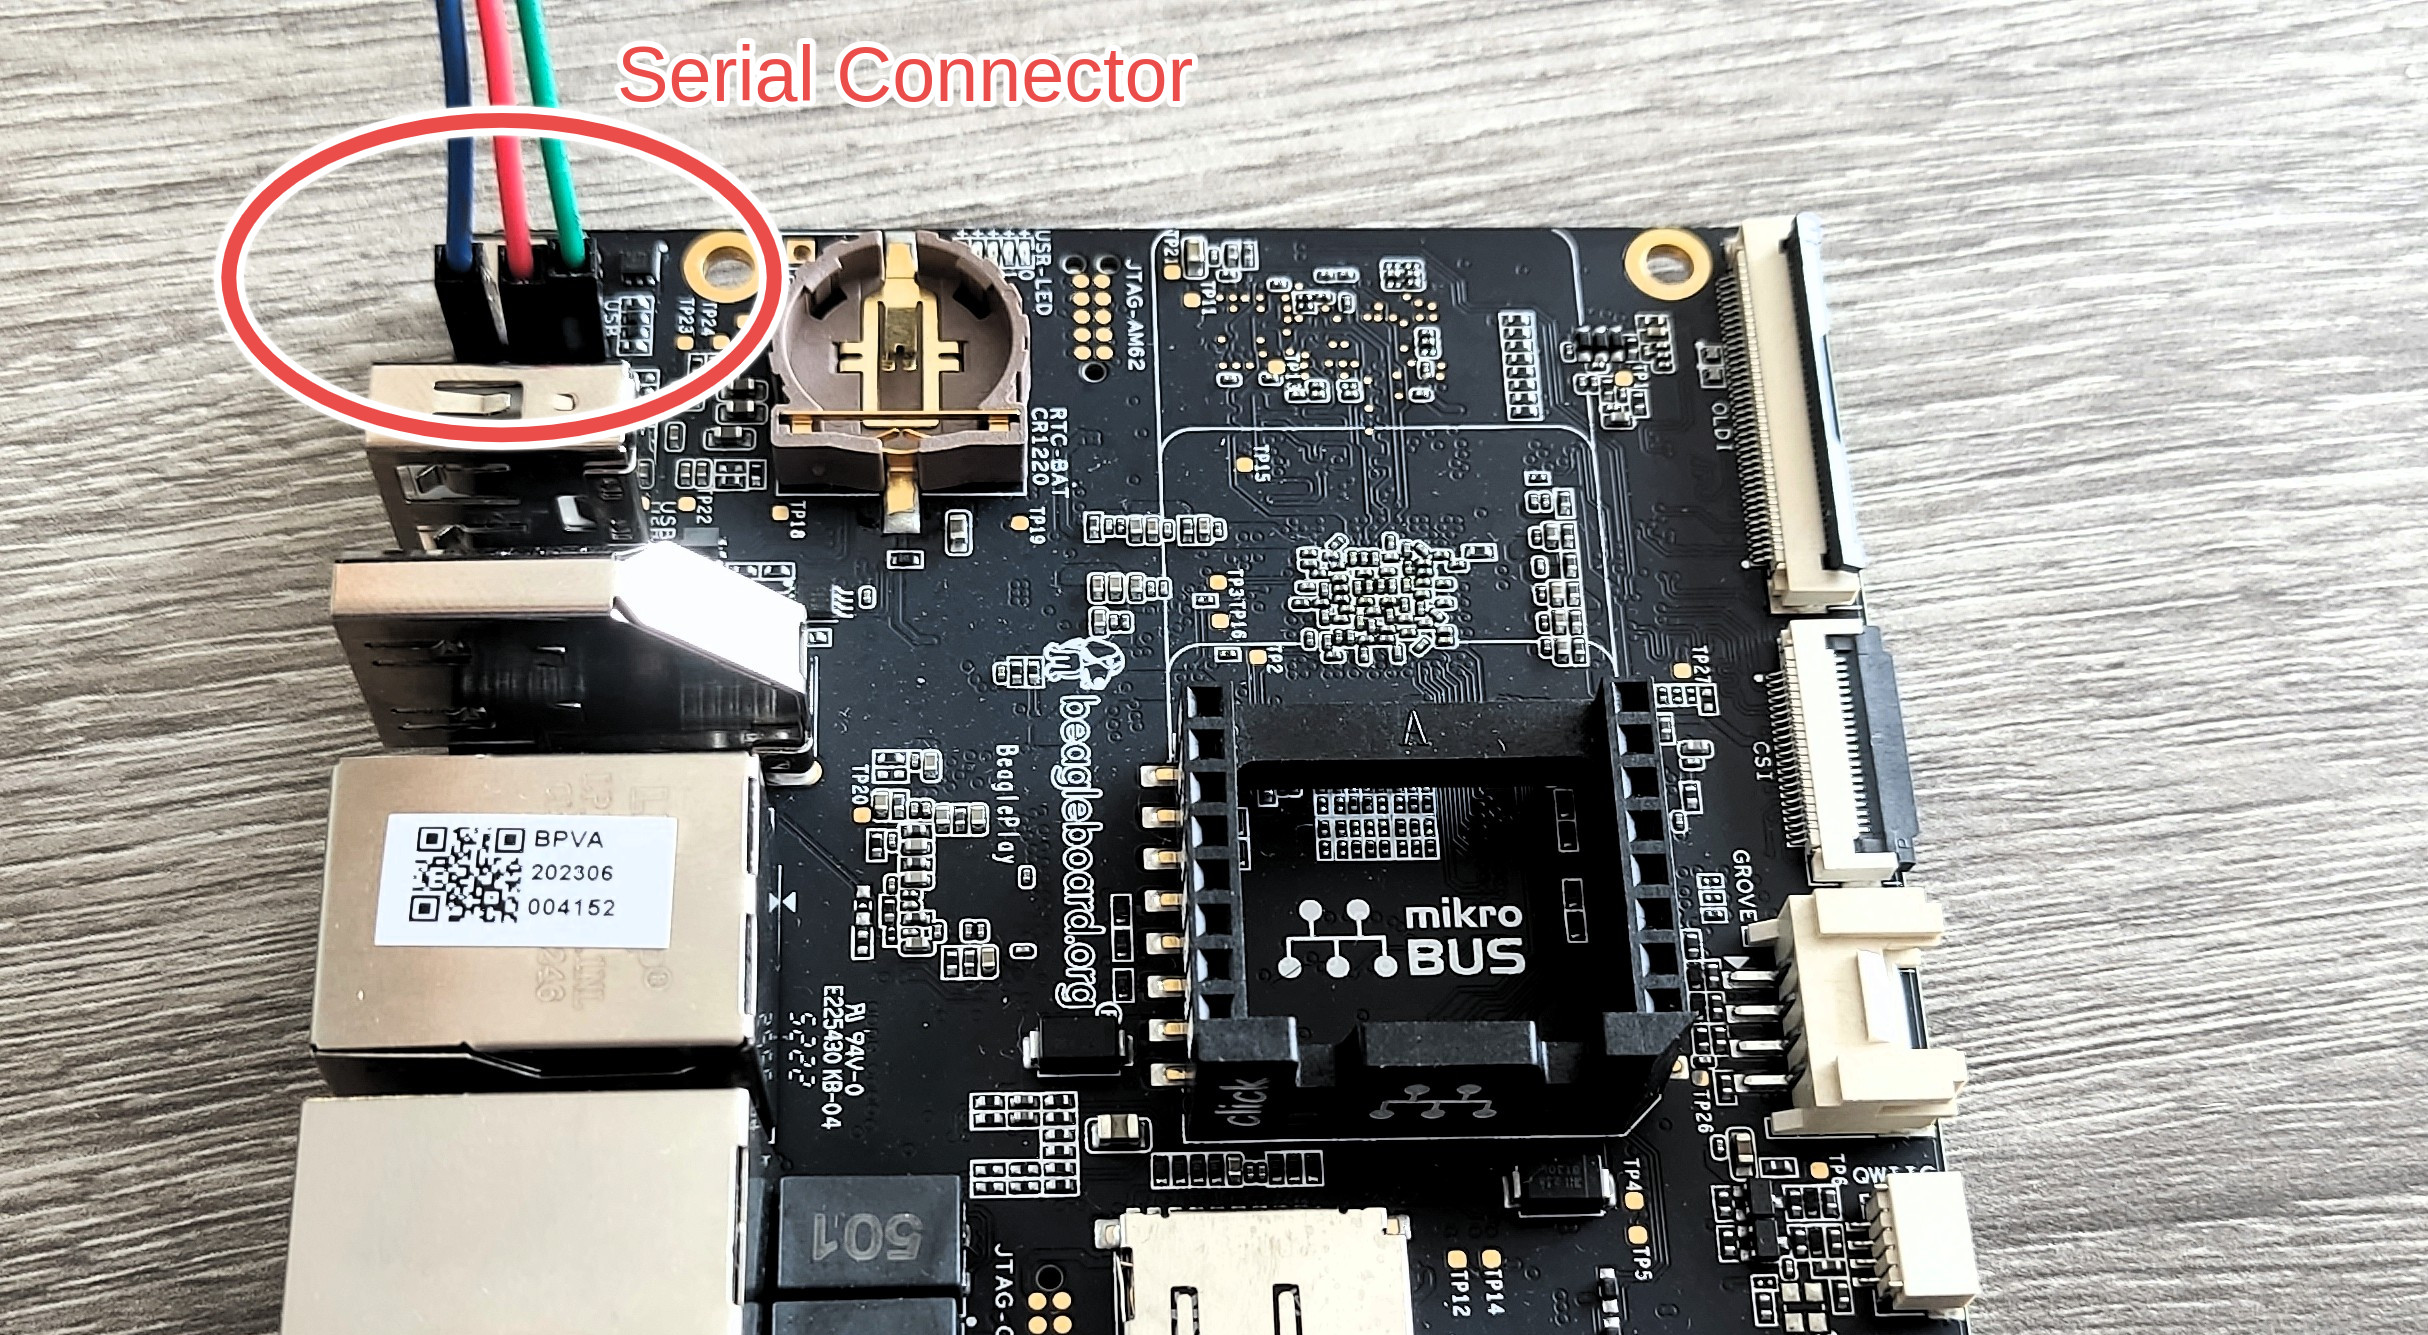
\includegraphics[width=8cm]{common/beagleplay-serial-connection.jpg}
\end{center}

Once the USB to Serial connector is plugged in, a new serial port
should appear: \code{/dev/ttyUSB0}.  You can also see this device
appear by looking at the output of \code{dmesg}.

To communicate with the board through the serial port, install a
serial communication program, such as \code{picocom}:

\begin{verbatim}
sudo apt install picocom
\end{verbatim}

If you run \code{ls -l /dev/ttyUSB0}, you can also see that only
\code{root} and users belonging to the \code{dialout} group have
read and write access to this file. Therefore, you need to add your user
to the \code{dialout} group:

\begin{verbatim}
sudo adduser $USER dialout
\end{verbatim}

{\bf Important}: for the group change to be effective, you have to
{\em completely log out} from your session and log in again (no need to
reboot). A workaround is to run \code{newgrp dialout}, but it is not global.
You have to run it in each terminal.

Now, you can run \code{picocom -b 115200 /dev/ttyUSB0}, to start serial
communication on \code{/dev/ttyUSB0}, with a baudrate of \code{115200}. If
you wish to exit \code{picocom}, press \code{[Ctrl][a]} followed by
\code{[Ctrl][x]}.

There should be nothing on the serial line so far, as the board is not
powered up yet.

Remove any SD card from the Beagle Play, we will be booting from the board's
eMMC.

It is now time to power up your board by plugging in the USB-C
cable supplied by your instructor to your PC.

See what messages you get on the serial line. You should see U-boot
start.

\section{Bootloader interaction}

Reset your board. Press the space bar in the
\code{picocom} terminal to stop the U-boot countdown. You should then see the
U-Boot prompt:

\begin{verbatim}
=>
\end{verbatim}

You can now use U-Boot. Run the \code{help} command to see the available
commands.

Type the \code{help saveenv} command to make sure that the
\code{saveenv} command exists. We use it in these labs to
save your U-Boot environment settings to the eMMC.

\begin{verbatim}
env default -f -a
saveenv
\end{verbatim}

If you don't have this U-Boot prompt, it's probably because you are doing these labs on your own
(i.e. without participating to a Bootlin course), you'll have to flash the eMMC
from recovery mode.

\subsection{Flashing the bootloader from recovery mode}

This section can be skipped if you already have a U-Boot prompt.

Follow the installation instructions at
\url{https://github.com/bootlin/snagboot} to install snagboot.

Make sure to install the snagboot udev rules as specified in the instructions:
\begin{verbatim}
$ snagrecover --udev > 50-snagboot.rules
$ sudo cp 50-snagboot.rules /etc/udev/rules.d/
$ sudo udevadm control --reload-rules
$ sudo udevadm trigger
\end{verbatim}

Go to the bootloader folder where boot images have been precompiled for you:

\begin{verbatim}
$ cd ~/__SESSION_NAME__-labs/bootloader
\end{verbatim}

Put the Beagle Play into recovery mode by unplugging and replugging the USB-C power
cable while pressing the USR button. Please beware that a warm reset performed
with the reset button won't work!

Wait about 10 seconds for the board's recovery mode to start, then check that
the following USB device is present:

\begin{verbatim}
$ lsusb | grep AM62x
Bus 003 Device 021: ID 0451:6165 Texas Instruments, Inc. AM62x DFU
\end{verbatim}

Run snagrecover:

\begin{verbatim}
# snagrecover -s am625 \
          -F "{'tiboot3': {'path': 'tiboot3.bin'}}" \
	  -F "{'tispl': {'path': 'tispl.bin'}}" \
	  -F "{'u-boot': {'path': 'u-boot.img'}}"
\end{verbatim}

After snagrecover is done, you should get a U-Boot console on the serial port.
Using this console, start DFU:

\begin{verbatim}
=> setenv dfu_alt_info '0=system raw 0 524288000;1=system raw 0 307133 mmcpart 1'
=> dfu 0 mmc 0
\end{verbatim}

Don't be upset by the following message, it's expected...

\begin{verbatim}
generic_phy_get_bulk : no phys property
\end{verbatim}

Then from the host, flash the image:

\begin{verbatim}
$ snagflash -P dfu -p 0451:6165 -D 1:tiboot3_emmc.bin -D 0:boot.img
\end{verbatim}

Once snagflash is done writing the boot image to eMMC, reset the board. You
should get a U-Boot prompt!

\section{Setting up networking}

The next step is to configure U-boot and your workstation to let your
board download files, such as the kernel image and Device Tree Binary
(DTB), using the TFTP protocol through a network connection.

For these next steps, make sure that your beagleplay board is directly connected
to your host PC through its ethernet port. If your computer already has a wired
connection to the network, your instructor will provide you with a USB Ethernet
adapter. A new network interface should appear on your Linux system.

\subsection{Network configuration on the target}

Let's configure networking in U-Boot:

\begin{itemize}
\item \code{ipaddr}: IP address of the board
\item \code{serverip}: IP address of the PC host
\end{itemize}

\begin{ubootinput}
=> setenv ipaddr 192.168.1.100
=> setenv serverip 192.168.1.1
\end{ubootinput}

Of course, make sure that this address belongs to a separate network
segment from the one of the main company network.

To make these settings permanent, save the environment:

\begin{ubootinput}
=> saveenv
\end{ubootinput}

\subsection{Network configuration on the PC host}

To configure your network interface on the workstation side, we need
to know the name of the network interface connected to your board.

Find the name of this interface by typing:

\begin{verbatim}
ip a
\end{verbatim}

The network interface name is likely to be
\code{enxxx}\footnote{Following the {\em Predictable Network Interface
Names} convention:
\url{https://www.freedesktop.org/wiki/Software/systemd/PredictableNetworkInterfaceNames/}}.
If you have a pluggable Ethernet device, it's easy to identify as it's
the one that shows up after pluging in the device.

Then, instead of configuring the host IP address from NetWork Manager's
graphical interface, let's do it through its command line interface,
which is so much easier to use:

\begin{verbatim}
nmcli con add type ethernet ifname en... ip4 192.168.1.1/24
\end{verbatim}

\section{Setting up the TFTP server}

Let's install a TFTP server on your development workstation:

\begin{verbatim}
sudo apt install tftpd-hpa
\end{verbatim}

You can then test the TFTP connection. First, put a small text file in
the directory exported through TFTP on your development
workstation. Then, from U-Boot, do:

\begin{ubootinput}
=> tftp 0x80000000 textfile.txt
\end{ubootinput}

The \code{tftp} command should have downloaded the
\code{textfile.txt} file from your development workstation into
the board's memory at location {\tt 0x80000000}\footnote{
This location is part of the board SDRAM. If you want
to check where this value comes from, you can check the SoC
datasheet at
\url{https://www.ti.com/lit/ug/spruiv7a/spruiv7a.pdf}.
It's a big document (more than 12,000 pages). In this document, look
for \code{Memory Map} and you will find the SoC memory map.
You will see that the address range for the memory controller
({\em DDR16SS0\_SDRAM})
starts at the address we are looking for.
You can also try with other values in the RAM address range.}.

You can verify that the download was successful by dumping the
contents of the memory:

\begin{ubootinput}
=> md 0x80000000
\end{ubootinput}

